\section{Losses in silica fibers}
Question: Elaborate on the reasons for losses in silica fibres. Plot typical spectral characteristic of power loss in silica fibers, indicate the transmission windows.\bigskip

Fibre power loss describes the proportion of beam power leaving the fibre to the power of introduced light beam. It is usually represented by a fiber attenuation coefficient:
\begin{equation}
    \alpha = \frac{10}{L}\log_{10}\left(\frac{P_{out}}{P_{in}}\right) \left[\frac{dB}{km}\right]
\end{equation}
where $L$ is the fibre's length. With its use the efficient power on a given length could be calculated as:
\begin{equation}
    P(L) = P(0)e^{-\alpha L}
\end{equation}

\begin{figure}[h]
    \centering
    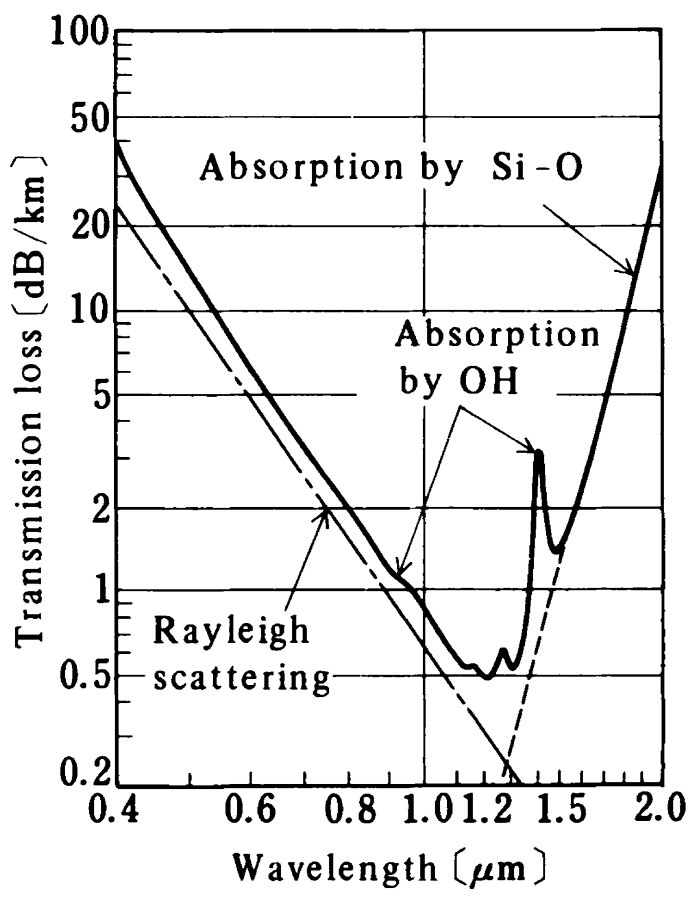
\includegraphics[width=0.5\textwidth]{images/losses.png}
    \caption{An example of the transmission-loss characteristics of low-loss optical fibres. Telecommunication windows visible here are $0.8\mu m$, $1.3\mu m$ and $1.55\mu m$. From~\cite{optfib}}
    \label{fig:my_label}
\end{figure}

Sources of these losses are manifold, but I will divide them here into three groups: (1) physical phenomena inherent to the silica, (2) impurities, (3) structural imperfections, both of internal and external origin.

\subsection{Inherent physical phenomena}

In the range from near ultra-violet to the far infra-red there are three main phenomena inducing power losses in the fibre: Rayleigh scattering, UV absorption and IR absorption.

The main cause of power losses in the visible spectrum is the Rayleigh scattering occurring due to the fluctuations of the refractive index\footnote{Of the order of $10^{-8}$.} throughout the core. These are introduced to the fibre in the manufacturing process during the glass solidification. Particles (atoms or molecules) several times smaller than the propagated wavelength can absorb the photon and re-radiate it in almost any direction. Rayleigh scattering increases towards the ultraviolet spectrum at $\approx\frac{1}{\lambda^4}$.

Photons of a sufficiently high energy, namely those of UV region, could be absorbed by the valence band electrons and excite them to the conductance band\footnote{Later this electron will emit a photon being a part of the scattered signal.}. 

In the infrared range the low-enegry photos are absorbed by the Si--O molecules and transformed into heat.

\subsection{Impurities}

Water and transition metal molecules are two important impurities introducing losses to the fibre. Hydroxyl OH group has a fundamental molecular vibration of $\lambda=2.8\mu m$ with second and third harmonics at 1.38 and 0.95$\mu m$. To suppress the second harmonic absorption below the SiO one, the water molecules cannot exceed 0.01 ppm.

In the past Cr, Mn, Co, Fe, Ni, Cu and V absorption was intensively observed, but today's good manufacturing process allows to ignore them.

\subsection{Structural imperfection}
Those may be constituted with the mechanical manipulation of the fibre such as bending, introducing geometrical  non-uniformity at the core-cladding boundary or with the imperfections at the connections (misalignment) and during the splicing.
